\documentclass[a4paper,10pt]{article}
\usepackage[utf8]{inputenc}
\usepackage{graphicx}
\usepackage{graphics}
\usepackage{color}
\usepackage{amsfonts}
\usepackage{amsmath}
\usepackage{booktabs}
\usepackage{CJKutf8}
\newcommand{\KZ}[1]{\textcolor{red}{Kenny: #1}}

\title{An Attention-based QA System for Medical Chatbot}
\author{Geng Xiaoqing}

\begin{document}

\maketitle

\begin{abstract}
Medical chat robot has always been regarded as an Information Retrieval Question Answering task. Instead of the widely used key-word based matching method, we propose a novel approach for open domain Question Answering using machine learning. We construct a model of attentive pooling LSTM network to calculate the pairwise similarity between a user input question and each standard question, then choose the question with the highest score as the question who has the same meaning with the input one. We perform an online A/B test with our new approach against the traditional key-word based one. Our experiment shows our NN-based method outperforms the traditional one in not only accuracy but also customers' feedback. Besides, we provide a Chinese medical QA dataset containing pairs of medical questions and answers for further usage. \KZ{I think we should rename
the title to ``question similarity computation in xxx''.}
\end{abstract}

\section{Introduction}
\KZ{I think you are implementing a QA system rather than a chat bot. A chat
bot has to manage more things such as state tracking. You can say your QA system
is a sub-system of a simple chatbot.} 

Open domain Question-Answering (QA) systems aim at delivering correct answers to questions posed in natural language. \cite{LearningToAnswerQuestions} QA is a well discussed problem with wide range of applications, such as online diagnosis and chatbots. When it comes to an enterprise chatbot, most methods are feature based, e.g. using key-word approaches. However, neural networks is showing advantages in static Question Answering tasks. In this paper, we propose a method using attentive pooling LSTM networks to implement a medical chatbot.

Our chatbot uses a Wechat Subscription for a local hospital as carrier. To support the chatbot, we have a standard QA library, in which the question-answer pairs are all designed by professional doctors. An example of the QA pairs is: 
\begin{center}
\begin{CJK}{UTF8}{gbsn}
\begin{tabular}{rl}
Q:&胎盘是什么 \\
A:&胎盘是个很奇妙的临时器官是母亲和胎儿交流交换对话的界面是胎儿 \\
  &生长发育的指挥中心是母亲保护胎儿免受外界有害物质伤害的屏障如 \\
  &果胎盘出了问题会导致一系列的不良后果 \\
\end{tabular}
\end{CJK}
\end{center}
The chatbot receives users' input questions then responds to them. There are three cases as for the chatbot's response.
\begin{itemize}
\item When the chatbot is confident enough to provide the user with exactly the correct answer, the chatbot directly answers the question and then suggests with some similar questions the user might be interested in. An example is ??????
\item When the chatbot is confused with several candidate answers and can't decide which one to choose, the chatbot replies with at most five candidate questions and asks the user which he or she meant. If the user choose one of the candidates questions, the chatbot then pushes the corresponding answer of the chosen candidate. An example is ????
\item When the chatbot is sure the answer to the user's question can't be found in the QA library, it directly tells the user it doesn't know the answer. An example is ???????
\end{itemize}
\KZ{It appears that these three cases translate into three difference thresholds
of similarity score. How to determine these thresholds and whether it is effective should be discussed later in the approach and evaluation.}

The back end of our chatbot uses a similarity score based method. When user inputs a question, for each standard question in the QA library, we calculate a similarity score between the standard one and the input one. Our system then regards the answer to the question with highest score as the correct answer. The similarity score is calculated by an attention-based LSTM network. Our network receives two sentences, a input user question and a standard question in the QA library, and returns a score presenting probability that the two sentences are talking about the same thing. We use attention mechanisms to let our network be aware of the content of the input pairs. Our system regards the standard question with the highest score as the one to be given to user.

Here are our main contributions.
\begin{itemize}
\item We provide a Chinese medical QA dataset, including a standard QA library, and clusters of similar questions collected from user data. There's no such datasets before our work.
\item We find out a better way to construct a enterprise chatbot. \KZ{It is
too strong to say this. We are *not* solving the chatbot problem; we merely
solved the question similarity problem.} Our NN-based method outperforms the key-word based one on our dataset. Besides, we perform an online A/B test with our NN-based approach against the mainstream keyword-based one, observing the correct answer rate and user interactions. The result shows NN-based chatbot does better in both indicators.
\end{itemize}

\KZ{Use references, not just fixed numbers below.}
The paper is organized as follows. In Section 2, we list the previous works on QA systems. Section 3 shows the definition and notations of the QA task.

\section{Related Work}
\KZ{You need to include more works on (short) text similarity or 
query similarity (query retrieval) here.  These are more relevant than QA.
Use the line break to separate the paragraphs instead of \textbackslash par.}

The mainstream of open-domain Question Answering uses feature based methods\cite{FeatureBased}. With the boost of machine learning, attempts to apply neural networks grow fast and they display great over-performance over the traditional methods in restricted-domain QA. For example, \cite{Yih2013} used Recurrent Neural Networks with lexical semantic resources; \cite{Wang2010} captured the alignment between sentence pairs by using a novel probabilistic model that models tree-edit operations.

More recently, deep learning methods achieved greater performance. In \cite{Yu2014,Feng2015,Severyn2015}, the authors used two vectors to present the question and answer independently, then calculate a relative score between the vectors which indicates the probability that the question and answer forms a correct pair.
\par Introducing attention to neural networks draws great attention these years. \cite{Cicero2016} applied the attention mechanism in answer selection. The authors added attention to the pooling layer to let the system be aware of the content of input question-answer pairs to improve performance. The two representation vectors of a pair of question and answer is determined not only by itself but also the other. Then a relative score is also calculated on them.
\par We follow \cite{Cicero2016} to use the attentive pooling LSTM networks in our task while change input. Since we have a standard QA library and user data, we regard the QA problem as a sentence similarity task and input to the system one user question along with a standard question from library. And the output of the system is a similarity score between the questions.
\par Our work significantly differs the above approaches in: 1) We do open-domain question answering, i.e. we do experiments online, while the above methods are all experimented in a restricted domain. 2) We use real data collected from user in a hospital WeChat official account to make the dataset, i.e. there are multiple possible questions asking for the same answer. While in above works, there is one-to-one correspondence between questions and answers.

\section{Problem Definition}
\KZ{In standard retrieval based QA, the problem is always reduced to a
text similarity problem. Bear this in mind.}
\par We treat the Question Answering problem as a sentence similarity task in a supervised learning setting. We have a set of standard question-answer pairs $\{(q_0,a_0),(q_1,a_1),...,(q_n,a_n)\}$, where $a_i$ is the correct answer to $q_j$ if and only if $i$ equals to $j$. Following \cite{Yih2013}, we denote user input questions $\{u_0,u_1,...,u_m\}$. Each $u_i$ is associated with a set of standard questions $\{(q_{i0},s_{i0}),(q_{i1},s_{i1}),...,(q_{in},s_{in})\}$, where $q_{ij}$ equals to $q_j$ in the standard pairs, and $u_i$ has the same meaning with $q_{ij}$ if and only if $s_{ij}=1$. Our goal is to learn a classifier on labelled user input question to predict the label $j$ of the new coming user question, and returns $a_j$ to user. To simplify the notations, we denote the input pair to the classifier each time $(u,q)$, indicating one user input question and one standard question.


\section{Attentive Pooling LSTM Networks}
\begin{figure}
\centering
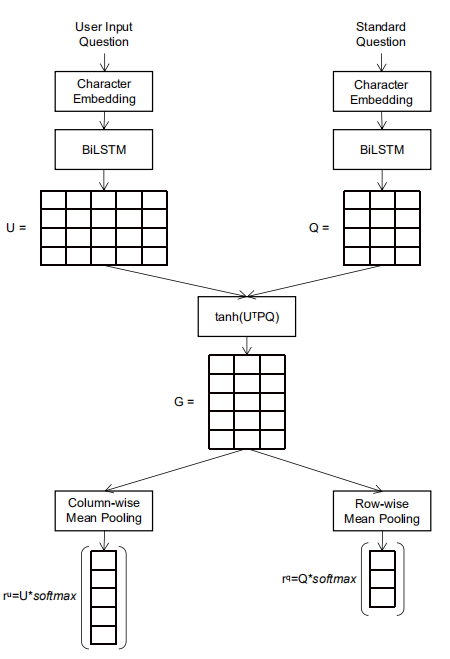
\includegraphics[width=0.75\textwidth]{model.png}
\caption{Attentive Pooling LSTM Networks}
\label{fig:model}
\end{figure}
\KZ{You need to say how this approach is different from other previous
text similarity approaches.}

\par Neural networks have been applied to QA tasks(cite!). Typically, a pair of question and answer is represented by two vectors independently and we score the correlation between them. Attention is a widely used mechanism to improve the performance of neural networks, which makes the networks know about the input pair. The representation of each sentence in the pair is influenced by one the other.  The overall framework is shown in Figure \ref{fig:model}. The input to the system is a pair of sentences, one user input question and one standard question. A bidirectional LSTM is applied to learn representations of each sentence. A matrix $G$ is to introduce attention mechanism. A similarity score is calculated on the two representations, and we regard the standard question with highest score as the target.  \cite{Cicero2016} used this network in restricted domain question answering and \cite{CunchaoTu} used it in network embedding.

\subsection{Character Level Embedding}
\par To get the reasonable representation of each character, we convert each character in the input sentences to a vector.
\par Given an one-hot encoded sentence $S=\{c^1,c^2,...,c^T\}$ with length $T$, for each element $c^i\in S$, only one dimension of the vector is set $1$, others $0$, i.e.,
\begin{equation}
c^i_j=
\begin{cases}
0,& i=j\\
1,& else
\end{cases}
\end{equation}
Since there are lots of characters, to distinguish different characters, $c^i$ is of extremely large dimension. To reduce the dimensionality, in the character embedding layer, each $c^i$ will be reduced to a new vector $e^i$, with $|e^i|<|c^i|$. The reduction procedure can be expressed as
\begin{equation}
e^i = W^{char}c^i
\end{equation}
where $W^{char}\in R^{d^c|V|}$ is a learnt matrix, $d^c$ is the hidden size of character embedding, $V$ is the set of all characters.
\par Thus, given sentence $S={c^1,c^2,...c^T}$ as input to the embedding layer, the output of this layer is $embed_s={e^1,e^2,...e^T}$.

\subsection{Bidirectional LSTM(BiLSTM)}
\par Long Short-Term Memory(LSTM) resolves the long-term dependency and gradient problems that traditional RNN has. An LSTM cell consists of several memory blocks, and there are three multiplication gates to control their activation states. The input gate($i$) controls the input information of the neuron. When the input gate is opened, new information is input into the neuron and the state of the neuron is updated. The output gate($o$) controls the output information of the neuron, and when the output gate is open, the information inside the neuron can be output and passed. The forget gate($f$) is to clean the information saved before in the neuron.
\par Given sequence $embed_s={e^1,e^2,...e^T}$, LSTM hidden size $d$, vector length $H$, the LSTM hidden vector $h_t$ at time $t$ is,
\begin{equation}
\begin{aligned}
i_t &= \sigma(W_i e^t + U_i h(t-1) + b_i) \\
f_t &= \sigma(W_f e^t + U_f h(t-1) + b_f) \\
o_t &= \sigma(W_o e^t + U_o h(t-1) + b_o) \\
\widetilde{C_t} &= \tanh(W_m e^t + U_m h(t-1) + b_m) \\
C_t &= i_t *\widetilde{C_t} + f_t * C_{t-1} \\
h_t &= o_t * \tanh(C_t)
\end{aligned}
\end{equation}
where $i$ represents the input gate, $f$ represents the forget gate, $o$ is the output gate, $C$ is neuronal memory vector, and $\sigma$ is the sigmoid function. $W\in R^{H \times d}$, $U \in R^{H \times H}$, $b\in R^{H \times 1}$ are all hyper parameters of the network.
\par The structure of LSTM makes it possible to solve the long-term dependency and gradient problems of ordinary RNN. However, since the text sequence goes through the neuron only in one way, the text in the preceding order can't catch the useful information that the subsequent text may bring to it, that is, the following information cannot be captured. Therefore, based on LSTM, BiLSTM was designed.
\par BiLSTM is bidirectional LSTM. The text is passed forward and reverse through the LSTM neurons. The output vector of BiLSTM is the concatenation of forward vector and inverse vector. At time $t$, the hidden vector $h_t$ of BiLSTM is,
\begin{equation}
h_t = \overrightarrow{h_t} || \overleftarrow{h_t}
\end{equation}

\subsection{Mutual Attention}
\par Mutual attention enables the pooling layer of biLSTM to be aware of the content of the input sequences. The representation of $u$ can be influenced by $q$ and vice versa.
\par The illustration of attention mechanism is shown in Figure \ref{fig:model}. Given the input pair $(u,q)$ of sequence length $l_u, l_q$ respectively, after computing $U\in \mathbb{R}^{w\times{l_u}}$ and $Q\in \mathbb{R}^{w\times{l_q}}$, we introduce matrix $G \in \mathbb{R}^{l_u \times l_q}$ to change the pooling layer of biLSTM. Matrix $G$ is computed as follows:
\begin{equation}
G = tanh(U^TPQ)
\end{equation}
where $P \in \mathbb{R}^{w\times w}$ is a matrix to be learned. Each element $G_{i,j}$ in $G$ indicates a correlation score between a pair of characters from $u$ and $q$ respectively.
\par Then, we conduct row-wise and column-wise pooling over $G$ to get two vectors $g^u \in \mathbb{R}^{l_u \times 1}$ and $g^q \ in \mathbb{R}^{l_q \times 1}$. We find out that mean pooling achieves best performance in our experiments. $g^u$ and $g^q$ are generated as follows:
\begin{equation}
\begin{aligned}
    &g^u_i = mean{(G_{i,1},G_{i,2},...,G_{i,l_q})} \\
    &g^q_i = mean{(G_{1,i},G_{2,i},...,G_{l_u,i})}
\end{aligned}
\end{equation}
\begin{equation}
    \begin{aligned}
        &g^u=[g^u_1,g^u_2,...,g^u_{l_u}]^T \\
        &g^q=[g^q_1,g^q_2,...,g^q_{l_q}]^T
    \end{aligned}
\end{equation}
\par For each element in $g^u$, $g^u_i$ indicates how close the $i^{th}$ character in $u$ is correlated to sequence $q$. The same is true with $g^q$.
\par After that, we apply softmax function to $g^u$ and $g^q$ and get $w^u \in \mathbb{R}^{l_u \times 1}$ and $w^q \in \mathbb{R}^{l_q \times 1}$:
\begin{equation}
    \begin{aligned}
    &w^u_i = \frac{exp(g^u_i)}{\sum_{j\in [1,l_u]}exp(g^u_j} \\
    &w^q_i = \frac{exp(g^q_i)}{\sum_{j\in [1,l_q]}exp(g^q_j}
    \end{aligned}
\end{equation}
\par For each element in $w^u$, $w^u_i$ indicates the weight, or importance, of the $i^{th}$ character in $u$ regarding $q$. The same is true with $w^q$.
\par Finally, the representations of $u$ and $q$ is computed as follows:
\begin{equation}
    \begin{aligned}
        &r^u=Uw^u \\
        &r^q=Q w^q
    \end{aligned}
\end{equation}
Thus the representation of $u$($q$) depends on not only $u$($v$) itself but also the other element in the pair.
\subsection{Scoring and Training Procedure}
\par For each pair of input $(u,q)$, a similarity score is computed. The higher the score is, the more similar the two sequences are. Given the representations $r^u$ for $u$ and $r^q$ for $q$, the similarity score between them is computed by cosine similarity:
\begin{equation}
    s_{u,q}=\frac{r^ur^q}{||r^u||\times||r^q||}
\end{equation}
\par To train the network, we introduce hinge loss here:
\begin{equation}
    Loss=max(0,m+s_{u,q_{pos}} - s_{u,q_{neg}})
\end{equation}
where $m$ is a manual constant margin, $q_{pos}$ and $q_{neg}$ are positive(correct) standard questions and negative(incorrect) ones.

\section{Experiments}
\par To prove the effectiveness of our system as a medical chat robot, we conduct both a static test and an online A/B test, and take both accuracy and user interaction info into account.
\subsection{Datasets}
\par We provide our own medical QA datasets.
\par \textbf{SomeName} is a library of 1600(?) standard question-answer pairs in raw Chinese. These questions cover congenital heart disease and gynecology, and the answers are provided doctors in hospitals.
\par \textbf{SomeNameAgain} contains questions asked by hospital chatbot users. Each user question is matched to a standard question in \textbf{SomeName}, indicating they are talking about the same thing. For concrete information see Table \ref{dataset}.
\KZ{Here you can give a few example similar questions.} 
\begin{table}[]
    \centering
\begin{tabular}{c|c|c}
    \toprule[1pt]
     Dataset & User questions & Average question length \\ \hline
     ?&?&? \\
     \bottomrule[1pt]
    \end{tabular}
    \caption{Statistics of Dataset}
    \label{dataset}
\end{table}

\subsection{Experimental Setup}
\KZ{This baseline is too weak. Should include a couple of stronger,
more recent approaches as comparisons.}
\subsubsection{Baseline}
\par We employ the traditional key-word based method as baseline:
\par \textbf{Term Frequency-Inverse Document Frequency(TF-IDF)} is a commonly used weighting technique in information retrieval and data mining. It is adopted to assess the importance of a word in a given task. The importance of a word increases proportionally with the number of times it appears in the file, but it also decreases inversely with the frequency it appears in the corpus.
\par In this paper, we adopt the TF-IDF method as baseline method to prove the effectiveness of our NN-based method in both static and online tests.


\subsubsection{Neural Network Settings}
\begin{table}[]
    \centering
    \begin{tabular}{c|c}
        \toprule[1pt]
         Dataset&? \\ \hline
         \#Qs in Train& ? \\ \hline
         \#Qs in Dev/Test& ? \\ \hline
         Char Embed Size& ? \\ \hline
         LSTM Hidden Size&? \\ \hline
         Matrix $P$ Shape&? \\ \hline Hinge Loss Margin&? \\ \hline
         Inital LR &? \\
        \bottomrule[1pt]
    \end{tabular}
    \caption{Neural Network Settings}
    \label{nnsetting}
\end{table}
\par To train our neural network, we select hyper-parameter values as Table \ref{nnsetting}.
\par \textbf{Character Embedding}. Our experiments show that character embedding performs better than word embedding. We train our character embedding directly on our dataset.
\par \textbf{Learning Rate}. We employ dynamic learning rate. Given initial learning rate $LR$, for the $e^{th}$ epoch, learning rate $lr_e$ is:
\begin{equation}
    lr_e = \frac{LR}{e}
\end{equation}

\subsubsection{Online A/B Test Settings}
\par A/B test is frequently applied when we have to choose the best solution from multiple ones. To conduct an A/B test, two solutions toward the same goal are proposed online. Users are randomly divided into two groups, using different solutions. The solution with better user feedback is considered better.
\par We conduct the A/B test between our NN-based approach and the key-word based baseline. We make the two methods online as the background program of a hospital chatbot on WeChat. We keep testing for 1 month. During testing, users are randomly divided into two groups, with their questions diverted to different systems.
\par To prove effectiveness, we record the following information during the A/B test.
\begin{itemize}
\item For those questions which are directly answered, manually label the user questions to get accuracy.
\item For those questions which are replied with several candidates, record the user's next input, which is a digital number. This number implies the user's choice of which candidate is the most similar to his or her question. The smaller the number, the better the performance. 
\item To prove user-friendliness and preference, we record interactions per use and using frequency of users. When the chatbot keeps giving wrong answers for several interactions, some users tend to say something bad to the robot. We also record this information as a criteria.
\item We call for some volunteers to try our system and record the comments.
\end{itemize}


\subsection{Experimental Results}
\subsubsection{Static Experimental Results}
\par We apply both our NN-based method and the baseline on our dataset. Results are shown in Table \ref{static}. We record accuracy at $k$, i.e. we consider it correct when the standard answer is ranked $r<k$.

\KZ{More discussion is needed here.}

\begin{table}[]
    \centering
    \begin{tabular}{c|c|c}
         \toprule[1pt]
         System & Acc at 1 & Acc at 5  \\ \hline
         NN-based & ? & ? \\ \hline
         Key-word based & ? & ? \\
         \bottomrule[1pt]
    \end{tabular}
    \caption{Accuracy of different systems}
    \label{static}
\end{table}
\par As the results show, the NN-based system outperforms the baseline.

\subsubsection{A/B Test Results}
\par We conduct the A/B test with our NN-based system against key-word based one for one month. Results are shown in Table \ref{abtest}.
\begin{table}[]
    \centering
    \begin{tabular}{c|c|c|c|c|c}
         \toprule[1pt]
         System&\#Users&Acc at 5&Interactions per use&Use frequency&Bad comments  \\ \hline
         & & & & & \\ \hline
         & & & & & \\
         \bottomrule[1pt]
    \end{tabular}
    \caption{A/B test results}
    \label{abtest}
\end{table}
\par Our system outperforms the baseline in:
\begin{enumerate}
    \item ...
\end{enumerate}

\section{Conclusion and Future Work}


\medskip

\bibliographystyle{unsrt}%Used BibTeX style is unsrt
\bibliography{sample}

\end{document}
